%%%%%%%%%%%%%%%%%%%%%%%%%%%%%%%%%%%%%%%%%%%%%%%%%%%%%%%%%%%%%%%%%%%%%%
%THINGS TO DO
%REPHRASE QUESTION
%EXPAND CONCLUSION
%ADD MORE STEPS FOR PROBLEMS
%

%%%%%%%%%%%%%%%%%%%%%%%%%%%%%%%%%%%%%%%%%%%%%%%%%%%%%%%%%%%%%%%%%%%%%%

\documentclass{article}
\usepackage[utf8]{inputenc}
\usepackage{graphicx}
\title{A Novel Solution To A Geometric Problem}
\author{Udit Gupta \and Matthew Zhang}
\date{November 2018}

\begin{document}

\maketitle


\section*{Introduction}
The following problem was presented as a challenge to all Centennial students.
\begin{center}
	How many ways can the angle theta be found?
	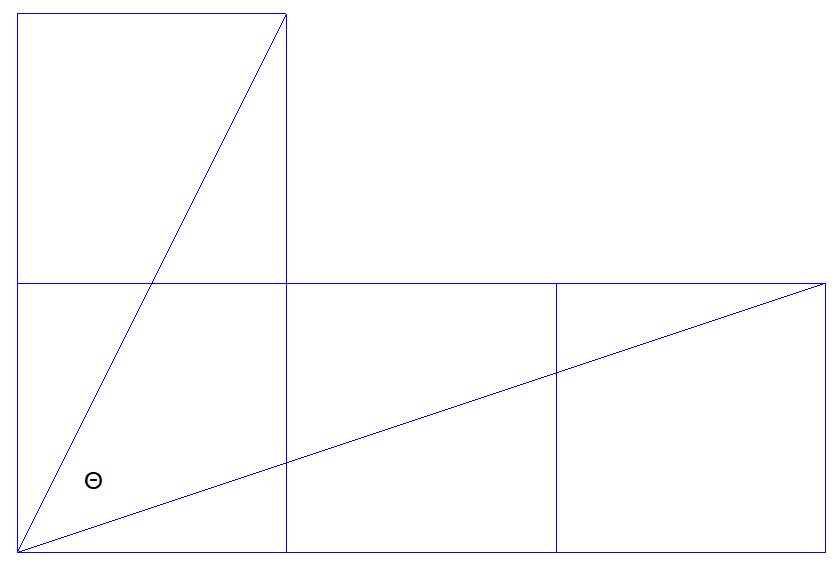
\includegraphics[width=.8\linewidth]{originalTheta.png}
\end{center}

\section*{Solution}
To begin, a Cartesian Plane is superimposed over the original diagram given alongside the challenge, with the bottom left corner as the origin.

Now, the side length of each square can be assumed to be some constant variable x.

\pagebreak

Utilizing this approach, a continuous function modeling the line segments can be generated. From the definition of slope as rise over run, the equations below can be formulated:
\newline

 Segment 1: $$ y=2x$$
 
 Segment 2: $$  y=\frac{1}{3}x$$
\begin{center}
	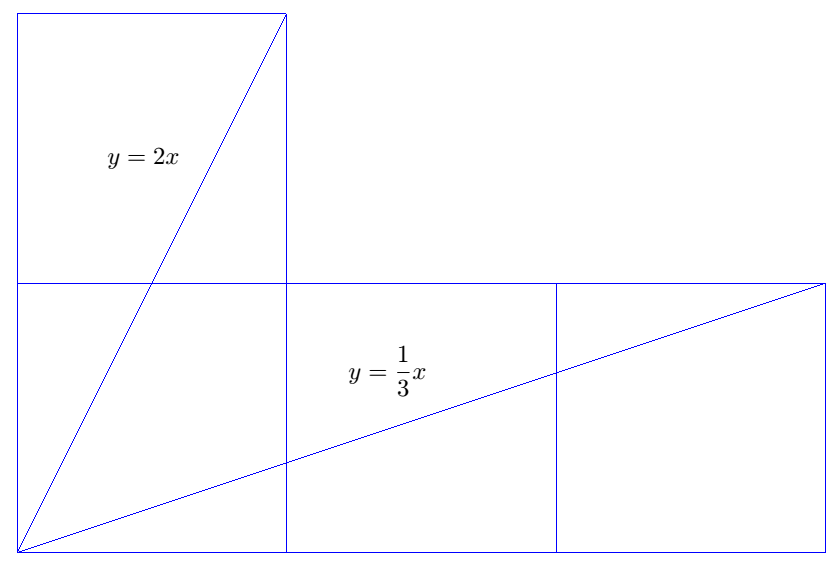
\includegraphics[width=.8\linewidth]{equations.png}
\end{center}

Now, a circle with radius r can be imposed $$x^2+y^2=r^2$$
\begin{center}
	\includegraphics[width=.8\linewidth]{circle.png}
\end{center}

\pagebreak
From here a chord is created connecting the intersections of segments 1 and 2 with the circle, henceforce referred to as chord $a$.
\begin{center}
	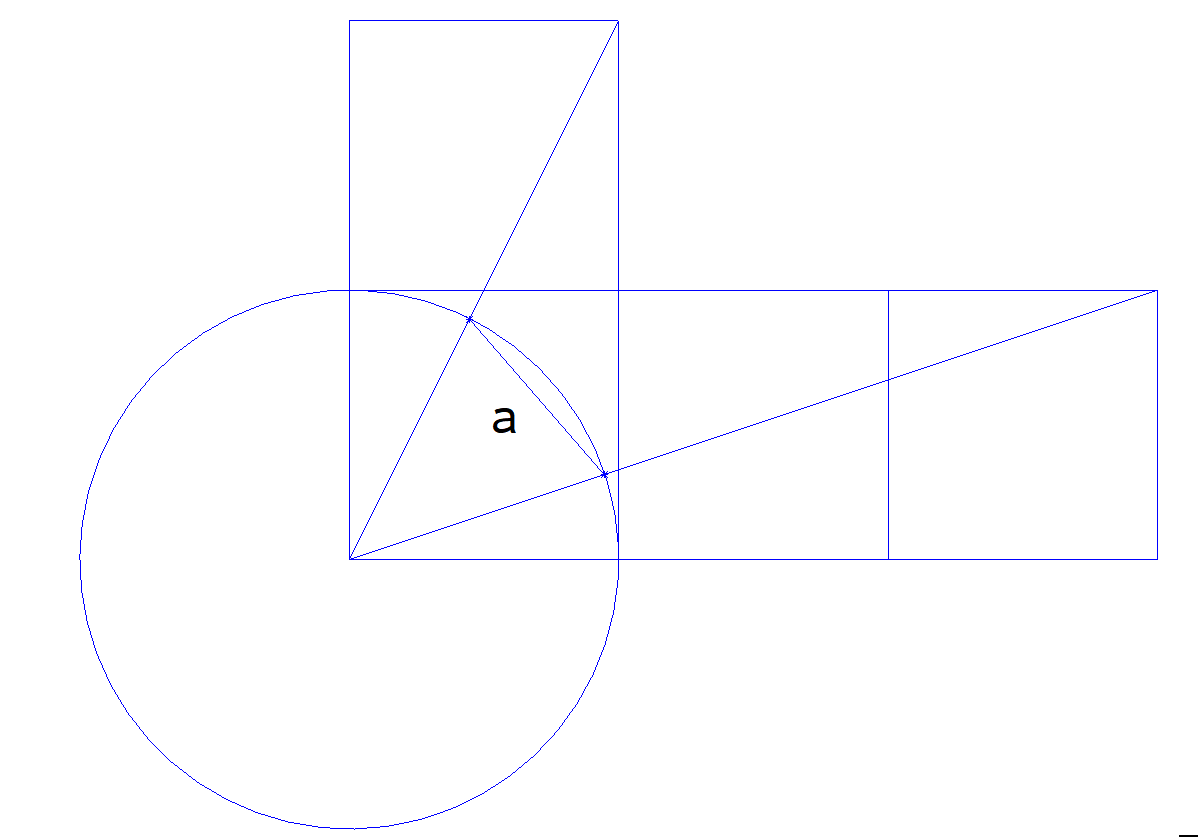
\includegraphics[width=.8\linewidth]{chord.png}
\end{center}

 Utilizing the distance formula, the distance of chord $a$ can be found, but first one must find the points of intersection. 

Using the equation for segment 1 and the equation for $a$ the circle, one can set up the following system of equations.
$$ y=2x $$
$$ x^2+y^2=r^2 $$
%%%%%%%%%%%%%%%%
%INSERT STEPS
%(SET UP SYSTEM AND SOLVE)
%%%%%%%%%%%%%%%%
Solving the system yields the point:
$$\bigg(\frac{ r\sqrt{5} }{5}, \frac{ 2r\sqrt{5} }{5}\bigg)$$
Doing the same for the other line gives us the following system:
$$ y=\frac{1}{3}x $$
$$ x^2+y^2=r^2 $$
Solving yields another point: 
%%%%%%%%%%%%%%%%
%INSERT STEPS
%(SET UP SYSTEM AND SOLVE)
%%%%%%%%%%%%%%%%
$$\bigg(\frac{3r\sqrt{10}}{10}, \frac{r\sqrt{10}}{10}\bigg)$$
Now, using the distance formula:
$$ a=\sqrt{\bigg(\frac{ r\sqrt{5} }{5}-\frac{3r\sqrt{10}}{10}\bigg)^2 + \bigg(\frac{ 2r\sqrt{5} }{5}-\frac{r\sqrt{10}}{10}\bigg)^2}$$
\newline
To avoid confusion, this solution will not be simplified.
By the law of cosines, the following expression is obtained.

$$ a^2=b^2+c^2-2bccos\theta$$

Where $a$ represents the length of the cord while $b$ and $c$ are the radius, $r$, of the circle. 

%%%%%%%%%%%%%%%%
%INSERT STEPS
%(PLUG VALUES AND SOLVE)
%%%%%%%%%%%%%%%%

Solving and simplifying this equation yields the solution:
 \begin{center}
$$\theta=45^o$$

\includegraphics[width=.8\linewidth]{solution.png}
 \end{center}

\end{document}
